%pdflatex --shell-escape --synctex=1 Diapo.tex

\documentclass[11pt, sans,xcolor=table]{beamer}
\usepackage[utf8]{inputenc}
\usepackage{default}
\usepackage{amssymb}
\usepackage{graphicx}
\usetheme{Warsaw}
\usepackage{animate}

%\usetheme{Malmoe}
%\usetheme{Copenhagen}
%\usetheme{Hannover}
%\usetheme{Goettingen}
%\usetheme{Antibes}
%\usetheme{AnnArbor}
%\usetheme{CambridgeUS}
%\usetheme{Dresden}

\title{Développement d'un jeu Bomberman sous Android et iOS}
\author{KLOB}
\institute{Université Montpellier II}
\subtitle{TER}

\begin{document}

\begin{frame}
\titlepage
\end{frame}


\begin{frame}{Sommaire}
\setcounter{tocdepth}{1}
\tableofcontents
\end{frame}

\section{Introduction}

\begin{frame}
\frametitle{Introduction}

	\begin{center} 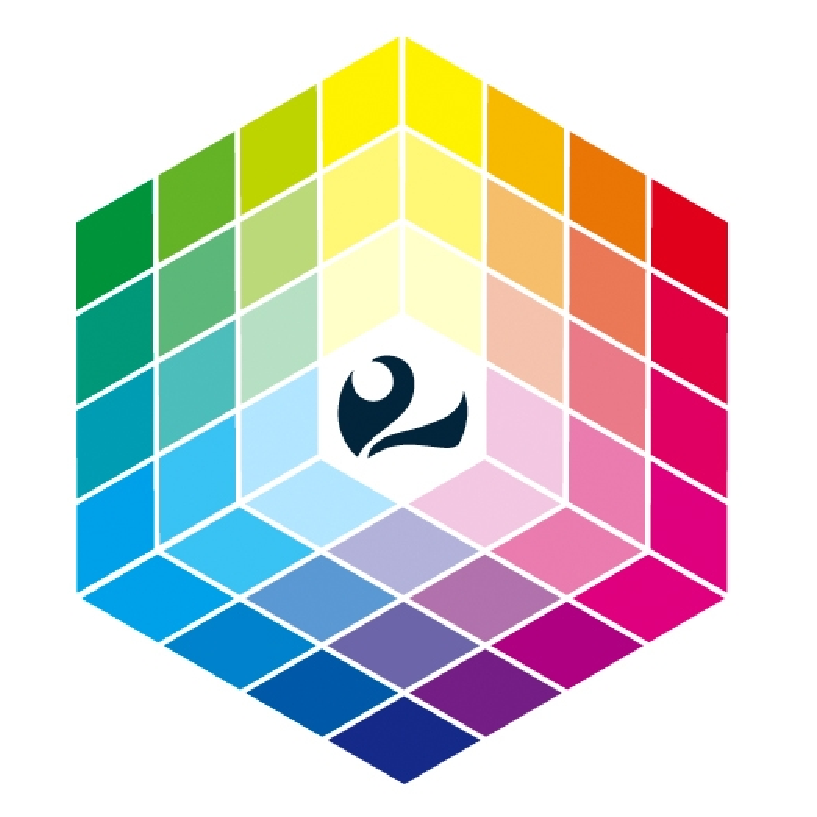
\includegraphics[scale=0.4]{img/logoUm2.eps} \end{center}

\end{frame}



\section{Présentation}

\subsection{Les jeux sur smartphone}

\begin{frame}
\frametitle{Présentation}
\framesubtitle{Les jeux sur smartphone}
Le marché des jeux vidéos sur console portable connait une réel expansion: \\ 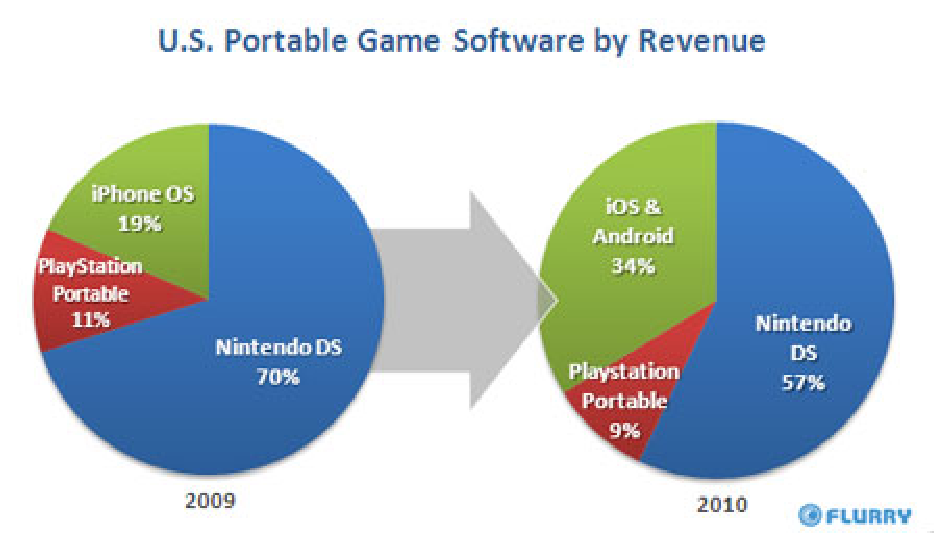
\includegraphics[scale=0.4]{img/marche_console_portable.eps} 

\begin{itemize} 
		\item{Coût peu couteux.}
		\item{Grand nombre de mini-jeux et de jeux.}
		\item{Public visé plus large.}
\end{itemize}
\end{frame}



%%%%%%%%%%%%%%%%%%%%%%%%%%%%%%%%%%%%%%%%%%%%
\subsection{Les sytèmes d'exploitations}


\begin{frame}
\frametitle{Présentation}
\framesubtitle{Android}

	\begin{minipage}{8cm}
		Le système d'exploitation possède : \\ 

	\begin{itemize} 
		\item Noyaux linux pour exploiter le matériel
		\item Librairies connues et open source (OpenGL ES, SQLite,...)
		\item Machine virtuelle Java (Dalvik virtual machine)
		\item API Java riche (package de Java SE, open source ou spécifique au système)
	\end{itemize}
	\end{minipage} & 
\includegraphics[scale=0.2]{img/android.eps} 

\end{frame}


%%%%%%%%%%%%%%%%%%%%%%%%%%%%%%%%%%%%%%%%%%%%


\begin{frame}
\frametitle{Présentation}
\framesubtitle{Android}
	\begin{minipage}{8cm}
	Les possibilités de développement sont: \\ 

	\begin{itemize}
		\item Langage principale Java, développement en C/C++ possible
		\item Kit de développement multiplateforme
		\item Développement sur téléphone ou sur émulateur
		\item Déploiement des applications peu coûteux
	\end{itemize}
	\end{minipage} & 
\includegraphics[scale=0.2]{img/android.eps} 
\end{frame}


%%%%%%%%%%%%%%%%%%%%%%%%%%%%%%%%%%%%%%%%%%%%


\begin{frame}
\frametitle{Présentation}
\framesubtitle{iOS}
	\begin{minipage}{8cm}
Le système d'exploitation possède : \\

	\begin{itemize} 
		\item Noyau hybride XNU dérivé de Mac OS X
		\item Librairies connues et open source (OpenGL ES, SQLite,...)
		\item Pas de machine virtuelle. Code compilé en C.
		\item API Objective-C riche (Core OS, Cocoa Touch,...)
	\end{itemize}
	\end{minipage} & 
\includegraphics[scale=0.2]{img/apple.eps} 
\end{frame}


%%%%%%%%%%%%%%%%%%%%%%%%%%%%%%%%%%%%%%%%%%%%


\begin{frame}
\frametitle{Présentation}
\framesubtitle{iOS}
	\begin{minipage}{8cm}
	Les possibilités de développement sont: \\ 

	\begin{itemize}
		\item Langage principale Objective-C, développement en C possible
		\item Kit de développement disponilbe sur Mac OS seulement
		\item Développement sur téléphone ou sur émulateur (nécessite un compte payant pour tester sur téléphone)
		\item Déploiement des applications coûteux
	\end{itemize}
	\end{minipage} & 
\includegraphics[scale=0.2]{img/apple.eps} 
\end{frame}


%%%%%%%%%%%%%%%%%%%%%%%%%%%%%%%%%%%%%%%%%%%%
\subsection{Le jeu Bomberman}


\begin{frame}
\frametitle{Présentation}
\framesubtitle{Le Bomberman}
\begin{minipage}{7cm}
Histoire
	\begin{itemize}
		\item Jeu d'action.
		\item Première sortie en 1987.
		\item Développé sur plusieurs consoles.
		\item Succès grâce au mode multijoueur sur certaines consoles.
	\end{itemize} \\
\end{minipage} & 
\includegraphics[scale=0.3]{img/bomberman1.eps} 

\end{frame}


%%%%%%%%%%%%%%%%%%%%%%%%%%%%%%%%%%%%%%%%%%%%


\begin{frame}
\frametitle{Présentation}
\framesubtitle{Le Bomberman}
Principe : \\ \\

\begin{minipage}{5cm}
	\begin{itemize}
		\item Le joueur incarne un poseur de bombes.
		\item But du jeu: détruire ses ennemis.
	\end{itemize} \\
\end{minipage} &  \begin{minipage}{5.5cm}
	\begin{itemize}
		\item Multiple bonus (Bonus de vie, de bombes, de vitesse,...).
		\item Multiple malus (Obligation de poser des bombes,...).
	\end{itemize} \\
\end{minipage} 

\begin{center} 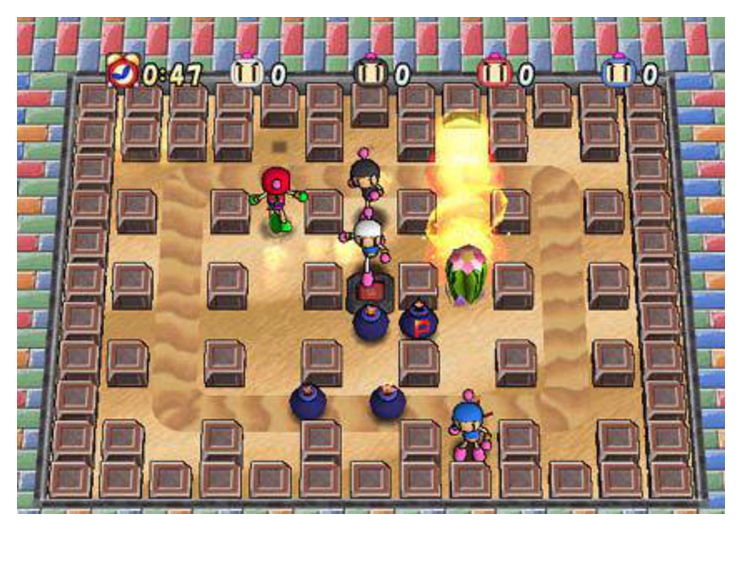
\includegraphics[scale=0.35]{img/bomberman2.eps} \end{center}

\end{frame}


%%%%%%%%%%%%%%%%%%%%%%%%%%%%%%%%%%%%%%%%%%%%
\subsection{Rapport avec l'enseignement}


\begin{frame}
\frametitle{Présentation}
\framesubtitle{Rapport avec l'enseignement}
Ce TER nous a permis de mettre en application les connaissances acquises dans nos parcours d'enseignements  pour: \\

	\begin{itemize}
		\item L'intelligence artificielle (parcours I2A).
		\item Les communications avec le serveur (parcours CASAR).
		\item L'utilisation de servlet (parcours DIWEB).
	\end{itemize} \\
	
\end{frame}





\section{Application}
\subsection{Lancement de l'application}

	\begin{frame}
	\frametitle{Application}
	\framesubtitle{Chargement de l'application}
	
	\begin{center}
		\begin{tabular}{cc}
			\begin{minipage}{5cm}
				\begin{block}{Lancement}
					\begin{itemize}
				 		\item Initialisation des données systèmes
			 		\end{itemize}
				\end{block}
			\end{minipage} &
			\begin{minipage}{8cm}
				 
\includegraphics[scale=0.3]{img/1.png} \\
			\end{minipage}\\
		\end{tabular}
		\end{center}

		
	
	\end{frame}
	
	\begin{frame}
	\frametitle{Application}
	\framesubtitle{Chargement de l'application}
		\begin{block}{Premier lancement}
			\begin{itemize}
			 	\item Copie des cartes officielles dans le repertoire du téléphone 
				\item Création et initialisation de la base de données SQLite
				\item Création d'un nouveau compte local
			\end{itemize}
		\end{block}
				
		\begin{block}{Lancement normal}
			\begin{itemize}
				\item Chargement de la base de données 
				\item Instantiation du dernier utilisateur
			\end{itemize}
		\end{block}
	
	\end{frame}
	
	
	\begin{frame}
	\frametitle{Application}
	\framesubtitle{Ecran d'accueil}
		\begin{center}
		\begin{tabular}{cc}
			\begin{minipage}{4cm}
		
				Menu d'accueil
				\begin{itemize}
					\item Partie locale
					\item Partie multijoueur
					\item Editeur de carte
					\item Options
					\item Choix compte local
					\item Ajout compte local
					\item Aide
				\end{itemize}
			\end{minipage}  &		
			\begin{minipage}{8cm}
				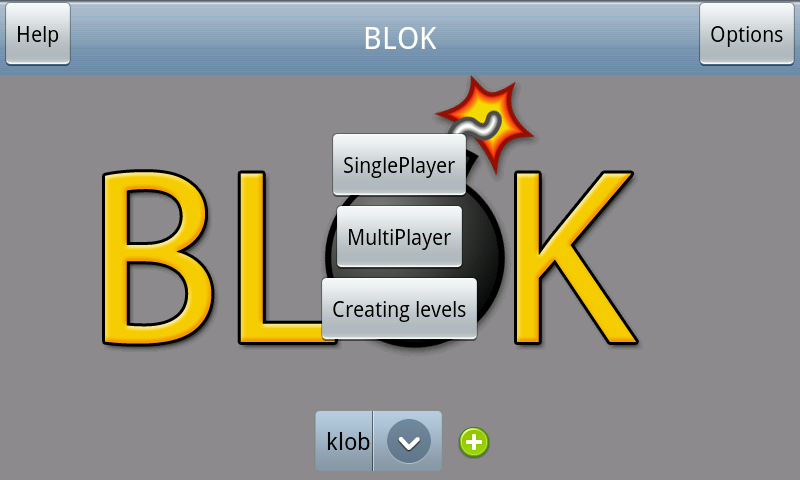
\includegraphics[width=6.5cm]{img/2.png} 
			\end{minipage}\\
		\end{tabular}
		\end{center}
	
	\end{frame}
	
	\begin{frame}
	\frametitle{Application}
	\framesubtitle{Les menus}
	
		\begin{block}{Objectifs:}
			\begin{itemize}
			  \item Interface claire
			  \item Facile d'utilisation
			  \item Navigation intuitive
			  \item Ergonomique
			\end{itemize}
		\end{block}
	\end{frame}
	
\subsection{Editeur de cartes}

	\begin{frame}
		\frametitle{Application}
		\framesubtitle{Editeur de cartes}
			\begin{center}
                             	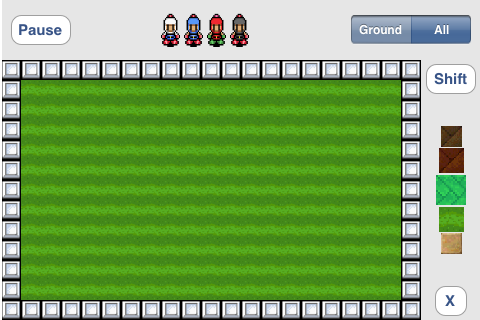
\includegraphics[width=7cm]{./img/img1.png}
               	\end{center}
	\end{frame}
	

	\begin{frame}
		\frametitle{Application}
		\framesubtitle{Moteur de rendu}
		
		
		Deux matrices:
		\begin{center}
               		\begin{tabular}{cc}
				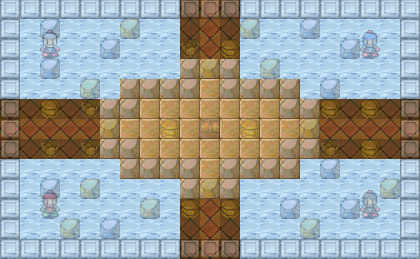
\includegraphics[width=4cm]{./img/img10.png} & 1er niveau \\
                                	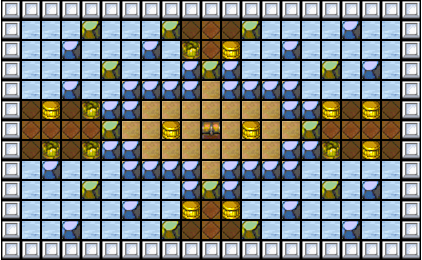
\includegraphics[width=4cm]{./img/img9.png} & 2ème niveau \\
               		\end{tabular}
               	\end{center}
	\end{frame}
	
	
	\begin{frame}
		\frametitle{Application}
		\framesubtitle{Interface Utilisateur}
		
		\begin{center}
               		\begin{tabular}{ll}
                       		\begin{minipage}{4cm}
					Différentes zones:
                                       	\begin{itemize}
                                   	 		\item Menu du haut
						\item La carte
						\item Menu droite
                                    		\end{itemize}
                       		\end{minipage}  &                
                       		\begin{minipage}{5.5cm}
                                		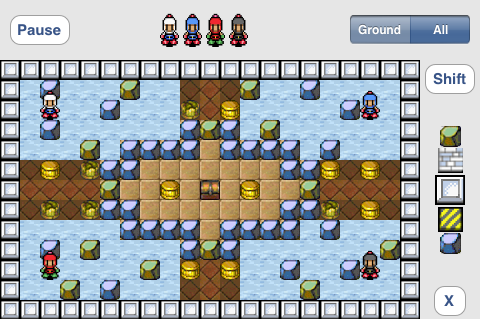
\includegraphics[width=5.5cm]{./img/img8.png}
                       		\end{minipage}\\
               		\end{tabular}
               	\end{center}
	\end{frame}
	
	
	\begin{frame}
		\frametitle{Application}
		\framesubtitle{Outils}
		
		Deux types de listes :
		
		\begin{center}
               		\begin{tabular}{p{3cm}p{3cm}}
				Sol & Blocs \\    
				\begin{minipage}{1cm}
                                		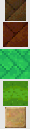
\includegraphics[scale=0.7]{./img/img4.png} \\
				\end{minipage}
				&
				\begin{minipage}{1cm}
                                		
\includegraphics[scale=0.7]{./img/img3.png} \\
				\end{minipage}
               		\end{tabular}
               	\end{center}
	\end{frame}
	
	
	\begin{frame}
		\frametitle{Application}
		\framesubtitle{Possibilités finales}
			\begin{center}
                             	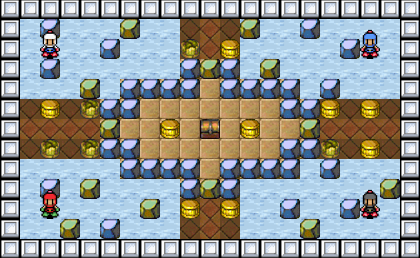
\includegraphics[width=7cm]{./img/img5.png}
               	\end{center}
	\end{frame}
	
	\begin{frame}
		\frametitle{Application}
		\framesubtitle{Menu}
		
		\begin{center}
               		\begin{tabular}{cc}
				\begin{minipage}{3cm}
                                       	\begin{itemize}
                                   	 		\item Reprendre
						\item Sauvegarder
						\item Réinitialiser
						\item Quitter
                                    		\end{itemize}
                       		\end{minipage}
				&
				\begin{minipage}{6cm}
					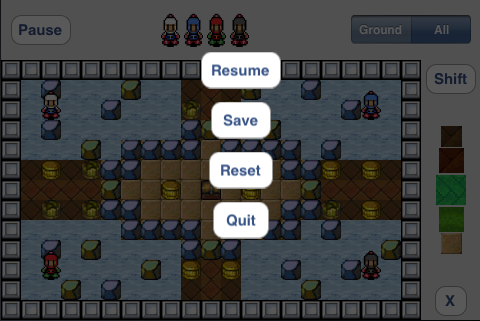
\includegraphics[width=6cm]{./img/img11.png}
				\end{minipage}
               		\end{tabular}
               	\end{center}
	\end{frame}

\subsection{Jeu}
	
	\begin{frame}
	\frametitle{Application}
	\framesubtitle{Création d'une partie solitaire}
	
		\begin{tabular}{cc}
			\begin{minipage}{5cm}
				Création d'une partie solitaire
				\begin{enumerate}
					\item Choix de la carte
					\item Type de la partie
					\item Difficulté des ennemis
					\item Nombre d'ennemis
					\item Temps de la partie
					\item Retourner à l'écran d'accueil
					\item Créer la partie
				\end{enumerate}
			\end{minipage} &
			\begin{minipage}{7cm}
				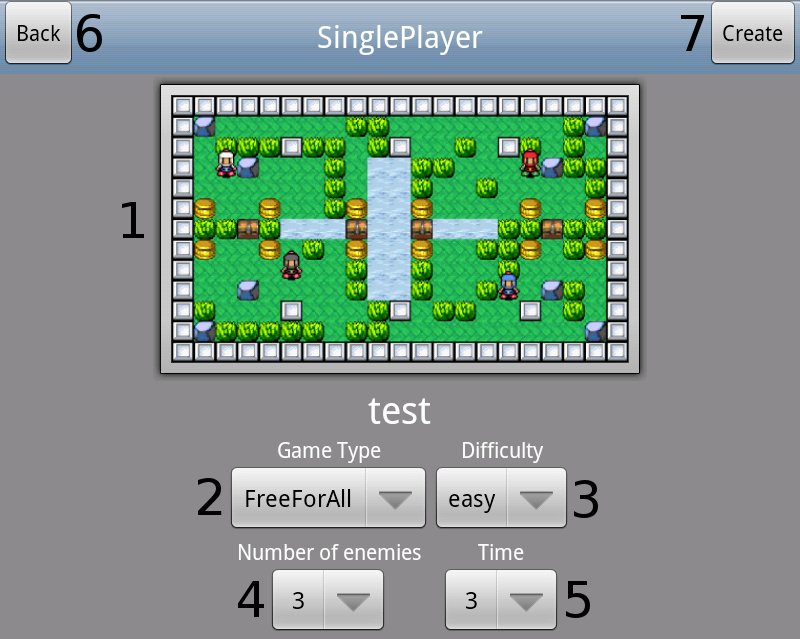
\includegraphics[width=6cm]{img/singleplayerbis.png} 
			\end{minipage}\\
		\end{tabular}
	
	\end{frame}
	

	\begin{frame}
	\frametitle{Application}
	\framesubtitle{Intelligence artificielle}
	
		\begin{tabular}{cc}
			\begin{minipage}{4cm}
				Niveaux de difficulté
				\begin{enumerate}
					\item Facile
					\item Moyen
					\item Difficile
				\end{enumerate}
			\end{minipage} &
			\begin{minipage}{6cm}
				
\includegraphics[width=6cm]{img/bots.png} 
			\end{minipage}\\
		\end{tabular}
	
	\end{frame}
	
	\begin{frame}
	\frametitle{Application}
	\framesubtitle{Pathfinding}
	
		\begin{tabular}{cc}
			\begin{minipage}{5cm}
				Algorithme A*
				\begin{enumerate}
					\item Heuristique (de Manatan)
					\item Coût de deplacement
					\item Premier chemin trouvé
					\item Rapidité (Dijskra)
				\end{enumerate}
			\end{minipage} &
			\begin{minipage}{5cm}
				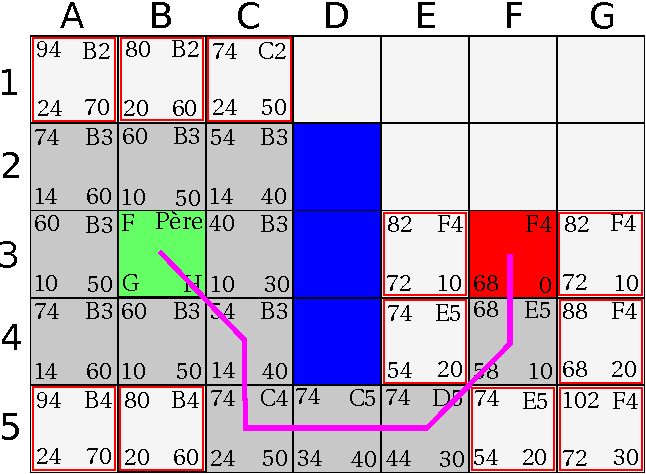
\includegraphics[width=6cm]{img/astar.png} 
			\end{minipage}\\
		\end{tabular}
	
	\end{frame}
	
	\begin{frame}
	\frametitle{Application}
	\framesubtitle{Pathfinding}
	
		\begin{tabular}{cc}
			\begin{minipage}{5cm}
				Algorithme de parcours en largeur
				\begin{enumerate}
					\item Pas de case d'arrivé necessaire
					\item Tous les chemins possibles
					\item Premier chemin trouvé
					\item Rapidité
				\end{enumerate}
			\end{minipage} &
			\begin{minipage}{5cm}
							\begin{center}
				\begin{tabular}{|c|c|c|c|c|c|c|} \hline
				\rowcolor{gray}  &  &                    &  &                  &  &                   \\\hline
				\cellcolor{gray} & \cellcolor{orange}1 $\leftarrow$ & \cellcolor{green}1 $\leftarrow$                   &&                && \cellcolor{gray} \\\hline
				\cellcolor{gray} & \cellcolor{orange}1 $\leftarrow$ & \cellcolor{gray}   & \cellcolor{gray} & \cellcolor{gray} &&	\cellcolor{gray} \\\hline
				\cellcolor{gray} & \cellcolor{orange}1 $\leftarrow$ & \cellcolor{orange}1 & \cellcolor{orange}1 $\rightarrow$ & \cellcolor{red}O                 && \cellcolor{gray} \\\hline
				\cellcolor{gray} & \cellcolor{orange}1 $\leftarrow$ & \cellcolor{gray}   & \cellcolor{gray} & \cellcolor{gray} && \cellcolor{gray} \\\hline
				\cellcolor{gray} & \cellcolor{red}O &                  &  &                && \cellcolor{gray} \\\hline
				\cellcolor{gray} && \cellcolor{gray}   && \cellcolor{gray} &&	\cellcolor{gray} \\\hline
				\cellcolor{gray} &&                  &&                && \cellcolor{gray} \\\hline
				\rowcolor{gray}  &  &                    &  &                  &  & \\\hline
				\end{tabular}
			\end{center}
			\end{minipage}\\
		\end{tabular}	
	
	\end{frame}
	
	\begin{frame}
	\frametitle{Application}
	\framesubtitle{Moteur de rendu}
	
		\begin{tabular}{ccccc}
			\begin{minipage}{3cm}
				\begin{center}
					Image
				\end{center}		
			\end{minipage} & &
			\begin{minipage}{2cm}
				\begin{center}
					Hashmap
				\end{center}
			\end{minipage} & &
			\begin{minipage}{3cm}
				\begin{center}
					Resultat
				\end{center}
			\end{minipage}\\
			\begin{minipage}{3cm}
				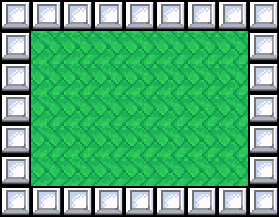
\includegraphics[width=3cm]{img/bitmap.png}
			\end{minipage} & + &
			\begin{minipage}{2cm}
				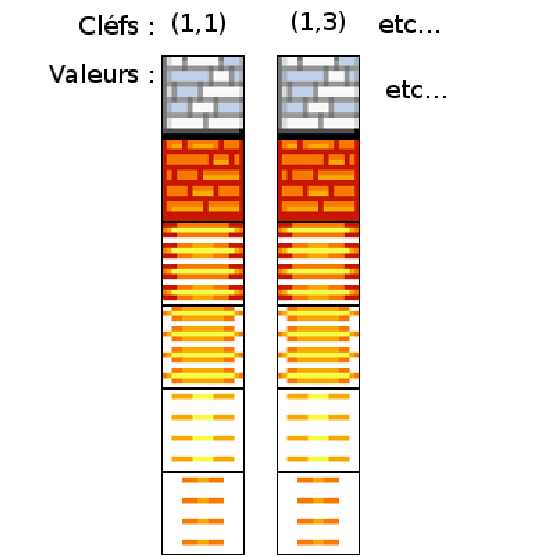
\includegraphics[width=3cm]{img/hashmap.png} 
			\end{minipage} & = &
			\begin{minipage}{3cm}
				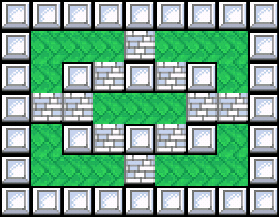
\includegraphics[width=3cm]{img/map.png} 
			\end{minipage}\\
		\end{tabular}
	
	\end{frame}
	
	\begin{frame}
	\frametitle{Application}
	\framesubtitle{Moteur Physique}
	
	\end{frame}
	
		\begin{frame}
	\frametitle{Application}
	\framesubtitle{Le jeu}
	
		\begin{tabular}{cc}
			\begin{minipage}{3cm}
				Ecran de jeu
				\begin{enumerate}
					\item 
				\end{enumerate}
			\end{minipage} &
			\begin{minipage}{7cm}
				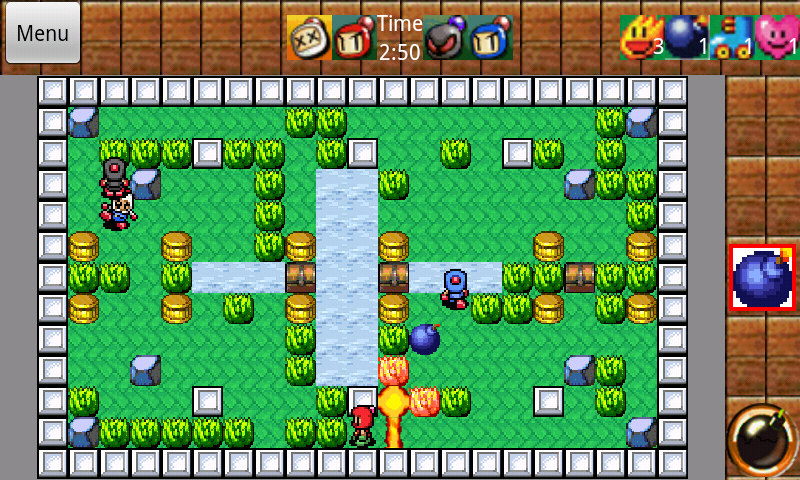
\includegraphics[width=8cm]{img/game.png} 
			\end{minipage}\\
		\end{tabular}
	
	\end{frame}
	
	\begin{frame}
	\frametitle{Application}
	\framesubtitle{Menu}
	
			\begin{tabular}{cc}
			\begin{minipage}{3cm}
				Menu
				\begin{enumerate}
					\item Reprendre
					\item Options
					\item Redemarrer
					\item Quitter
				\end{enumerate}
			\end{minipage} &
			\begin{minipage}{8cm}
				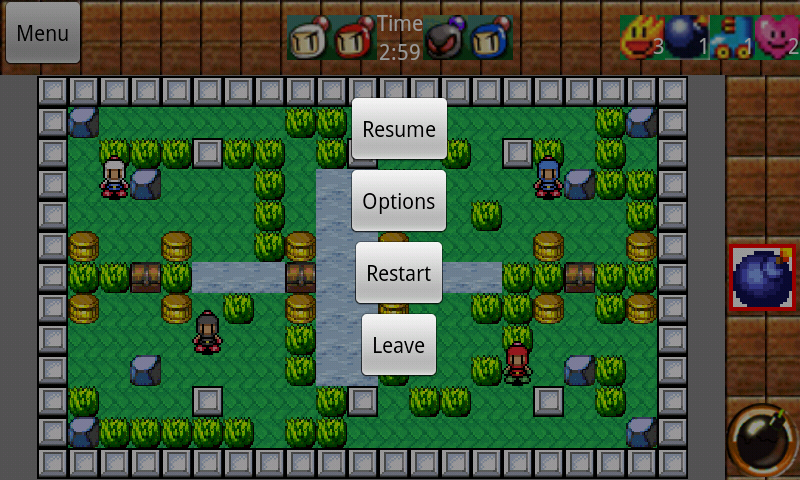
\includegraphics[width=8cm]{img/menusolo.png} 
			\end{minipage}\\
		\end{tabular}
	
	\end{frame}

\subsection{Reseau}

\begin{frame}
\frametitle{Application}
\framesubtitle{Fonctionnalités}

	\begin{center}
		\begin{tabular}{cc}
			\begin{minipage}{4cm}
				Les joueurs ont accès à:
				\begin{itemize}
				  \item la création de comptes multijoueurs
				  \item la page de connexion en ligne
				  \item la liste des parties en lignes
				\end{itemize}
				\end{minipage}&		
				
			\begin{minipage}{8cm}
				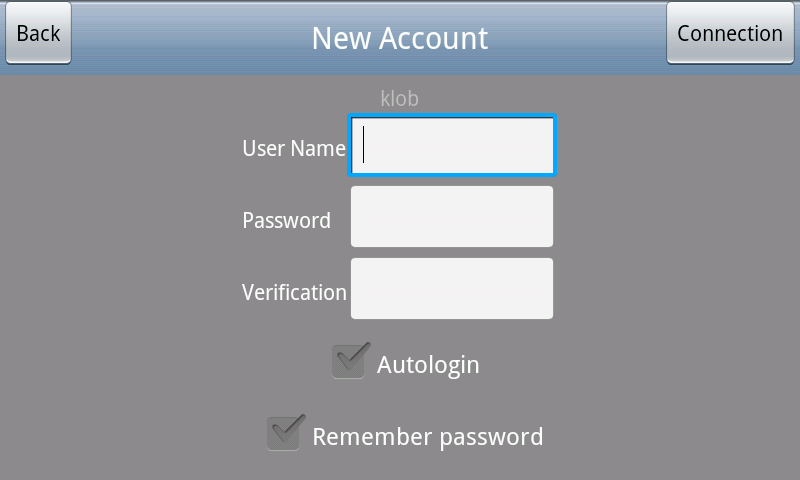
\includegraphics[width=7cm]{img/3.png} 
			\end{minipage}\\
			
			
			\end{tabular}
	\end{center}
	

\end{frame}

\begin{frame}
\frametitle{Application}
\framesubtitle{Outils}
	\begin{center}
		\begin{tabular}{cc}
			\begin{minipage}{7cm}
			
			\begin{block}{Outils utilisés: }
				\begin{itemize}
				  \item Servlets
				  \item Serveur d'application
				  \item JSON
				  \item SQLite
				\end{itemize}
			\end{block}
			
			\end{minipage}&
			
			\begin{minipage}{4cm}
				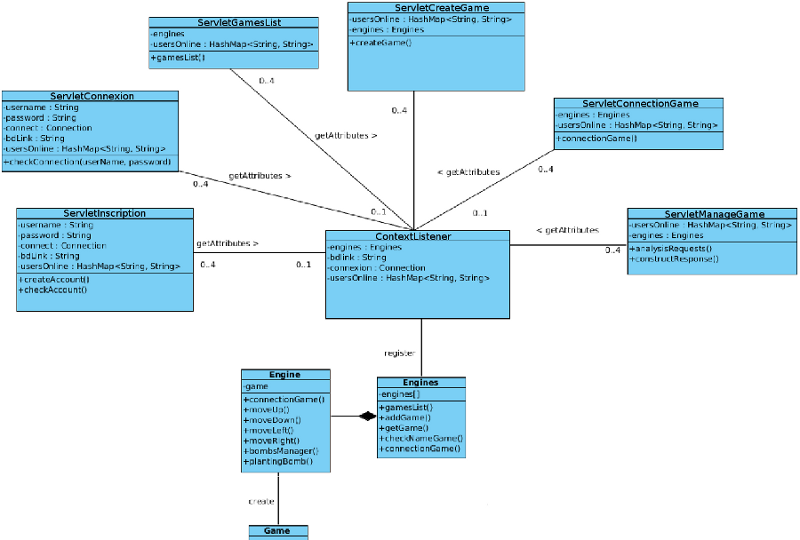
\includegraphics[scale=0.5]{img/serveur.png} 
			\end{minipage}\\
				
			\end{tabular}
	\end{center}
			
\end{frame}


\begin{frame}
\frametitle{Application}
\framesubtitle{Principe}

	\begin{center}
		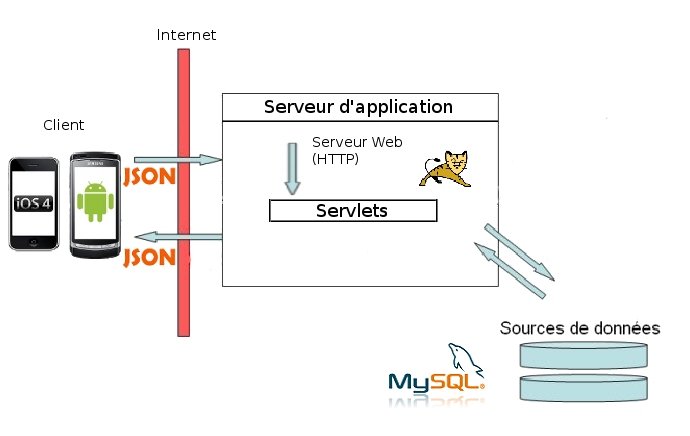
\includegraphics[width=9.4cm]{img/4.png} 
	\end{center}
	

\end{frame}


\section{Généralités}

	Il nous a paru important lors de la réalisation de ce projet
	de mettre au point un code facilement améliorable et surtout
	réutilisable par les personnes qui souhaiteraient personnaliser
	le jeu à leur façon.
	
	C'est pourquoi un des points primordial à été tout d'abord de
	rédiger notre code ainsi que notre documentation totalement 
	en anglais afin qu'une majorité de personne puissent les comprendre.

\section{Client}

	\subsection{Modèles de conception}
	
		\subsubsection{MVC}
		
			Le \gls{mvc} est une architecture et une méthode de
			conception qui organise l'\gls{ihm} d'une 
			application.
			Pour cela, il divise l'\gls{ihm} en un modèle (modèle de données),
			une vue (présentation, interface utilisateur) et un contrôleur
			(gestion des événements, synchronisation), chacun ayant un rôle
			précis dans l'interface.
			
			\begin{center}
				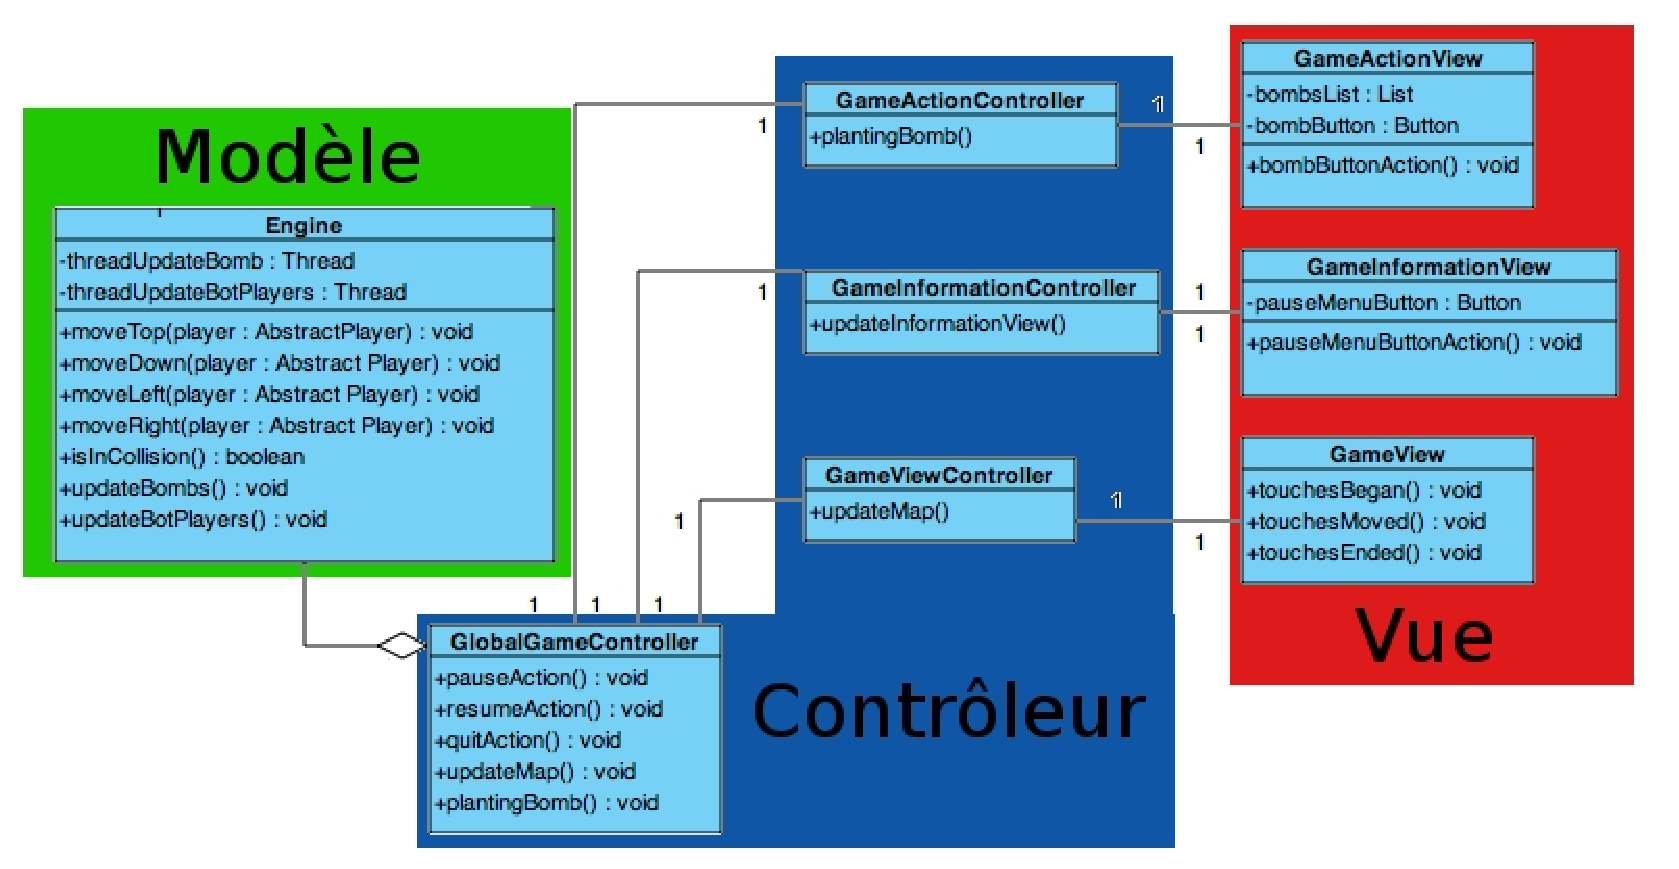
\includegraphics[width=11cm]{./Reutilisabilite/Img/mvc.eps}
			\end{center} 
			
			L'avantage de cette méthode de conception est qu'elle permet la
			modification d'une des parties sans affecter les autres.
			Il serait dans notre cas possible de pouvoir modifier le gameplay,
			l'interface graphique ou encore d'améliorer le moteur du jeu sans pour
			cela devoir s'occuper du reste du code.		
		
		\subsubsection{Design Pattern Décorateur}
		
			\begin{center}
				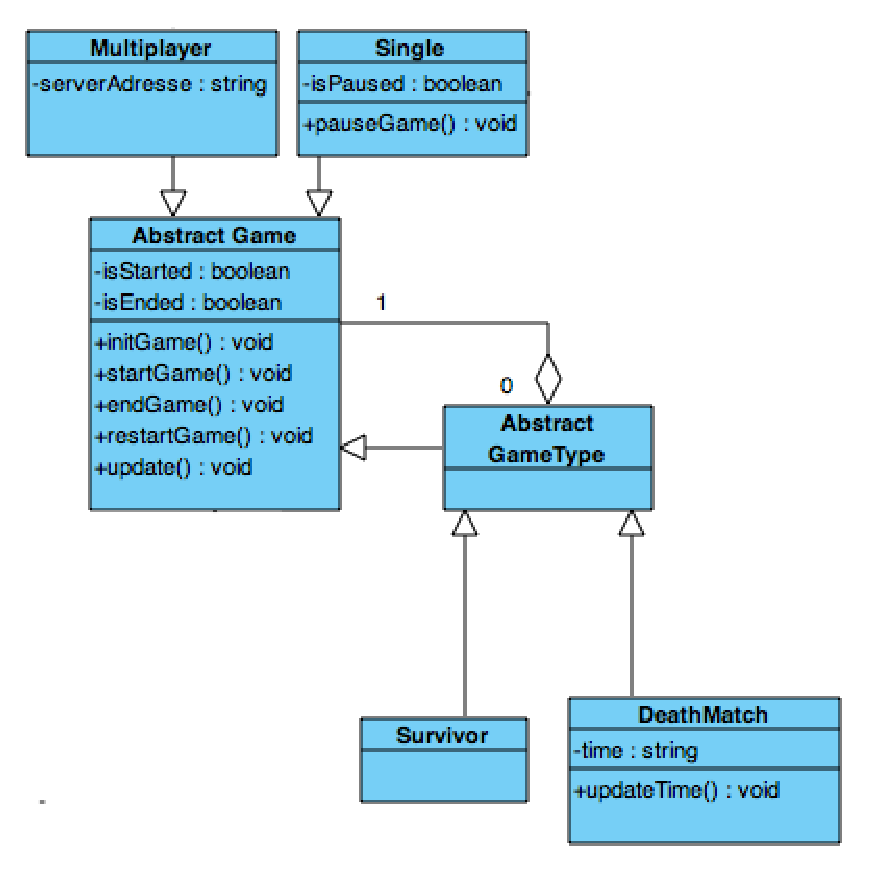
\includegraphics[width=11cm]{./Reutilisabilite/Img/decorateur.eps}
			\end{center} 
		
	\subsection{XML}
	
		Le fait d'avoir utilisé le \gls{xml} permet de pouvoir modifier les diverses caractéristiques de nos
		ressources sans necessiter la moindre modification du code source.
	
		\subsubsection{Internationalisation}
		
			Dans notre jeu, nous avons pris en charge le support de l'internationalisation.
			Pour cela, nous avons décidé de créer pour chaque langue un fichier
			\gls{xml} contenant la globalité des mots apparaissant dans notre application.
			Si l'utilisateur souhaite rajouter une nouvelle langue, il lui suffira d'ajouter
			un fichier \gls{xml} dans le répertoire correspondant à la langue voulu et d'y traduire
			tous les mots présents dans les \gls{xml} des langues déjà existants.
	
		\subsubsection{Personnalisation}
	
			Là aussi, l'utilisation du \gls{xml} montre ses avantages lors de la personnalisation
			des diverses ressources mises à disposition de l'utilisateur.
			
			Prenons par exemple le code \gls{xml} d'un objet indestructible :
			
			$\,$
		
			\begin{footnotesize}
				\lstset{tabsize=1, frame=shadowbox, rulesepcolor=\color{gray}}
				%\lstinputlisting{./Reutilisabilite/code/objects.xml}
			\end{footnotesize}
			
			Si l'on souhaite associer un son à cet objet, il suffit d'éditer l'attribut \emph{sound}
			et de rajouter le nom de celui que l'on souhaite.
			Il en est de même pour les différentes caractéristiques de notre objet.		

\section{Serveur}

	\subsection{Modèles de conception}
	Tout comme le côté client, l'architecture du serveur utilise le pattern
	décorateur. Ce dernier permettra de rajoûter des types de parties officielles,
	et concernera donc toutes les parties multijoueurs.
	
	\subsection{Fonctionnalités}
	En ce qui concerne les fonctionnalités, là aussi il est facilement possible de
	les étendres. En effet à chaques servlet correspond une fonctionnalité, il 
	sera seulement nécessaire de créer de nouvelles servlet, et de les incorporer
	au serveur.
	
	La base de données peut elle aussi être complété par exemple par la sauvegarde
	de scores d'utilisateurs et permettre le partage. En fait étant donné sa
	simplicité, un rajoût de table de manière raisonné et réfléchie, est facilement
	envisageable.	
	

	\subsection{Servlets}

\section{Discussion}

	\subsection{Difficultés}
		\begin{frame}
			\frametitle{Discussion}
			\framesubtitle{Difficultés}
				\begin{tabular}{cc}
					Android & iOS \\
					\begin{minipage}{5cm}
						\begin{itemize}
							\item Nouvelle plate-forme
							\item Multi-touch
							\item Ressources limitées
						\end{itemize}
					\end{minipage}
					&
					\begin{minipage}{5cm}
					\begin{itemize}
						\item Nouveau langage (Objective-C)
						\item Nouvelle plate-forme
						\item Gestion manuelle de la mémoire
						\item Ressources limitées
					\end{itemize}
				\end{minipage}
			\end{tabular}
		\end{frame}
		
		
	\subsection{Problèmes}
		\begin{frame}
			\frametitle{Discussion}
			\framesubtitle{Problèmes}
			Android et iOS :
			\begin{itemize}
				\item Tester l'application
				\item OpenGL ES
			\end{itemize}
		\end{frame}
		
		
	\subsection{Améliorations}
		\begin{frame}
			\frametitle{Discussion}
			\framesubtitle{Améliorations}
			\begin{itemize}
				\item Mode histoire
				\item Ajout de bonus / malus
				\item Rajout de types de parties
			\end{itemize}
		\end{frame}


\section{Conclusion}

\begin{frame}
\frametitle{Conclusion}
\framesubtitle{Apports en relation avec nos parcours d'enseignement}
\begin{tabular}{c|c|c|c}

I2A & CASAR & DIWEB & GL \\\hline
Recherche   &  Communication  &  Servlet  & Conception d'une  \\
 opérationelle  & mobile-serveur &   & application \\
                           &                              &                &                   \\
A* & Mise en place  & BDD & MVC \\
      &d'un serveur & & \\
                           &                              &                &                   \\
Parcours  &  Sécurisation   & XML  & Design pattern  \\
en largeur & du réseau & & décorateur \\

                           &                              &                &                   \\

Moteur de jeu & & IHM  & \\
           &           &        ergonomique        &        \\

\end{tabular}

\end{frame}



\begin{frame}
\frametitle{Conclusion}
\framesubtitle{Ce que cela nous a apporté}
\begin{itemize}
	\item Découverte de la programmation mobile (SDK Android, SDK iOS).
	\item Apprentissage d'un nouveau langage (Objective-C).
	\item Découverte de la programmation de jeux vidéos.
	\item Communication mobile-serveur.
	\item Travail en groupe.
\end{itemize}
\end{frame}



\end{document}